\documentclass{beamer}

%%%%%%%%%%%%%Solarized Theme%%%%%%%%%%%%%%%
\usecolortheme[light, accent=cyan]{solarized}
\beamertemplatenavigationsymbolsempty

%%%%%Packages%%%%%
\usepackage{graphicx}
\graphicspath{ {static/} }

\usepackage{hyperref}
\usepackage{colortbl, xcolor}
\usepackage{booktabs}

\usepackage{tikz}
\usepackage{standalone}
\usetikzlibrary{shapes.multipart}

\usepackage{amsmath}
\usepackage{amsthm}
\usepackage{amssymb}
\usepackage[framemethod=TikZ]{mdframed}
\setbeamertemplate{blocks}[default]

%%%%%%Title%%%%%%%%
\title{\textbf{GAME THEORY}}
\date{\textbf{Full STEAM Ahead 2018}}

\begin{document}

\maketitle

\begin{frame}
    \centering
    
\includegraphics[width=.2\textwidth]{players} \hspace{.6cm}
    
\includegraphics[width=.2\textwidth]{actions} \hspace{.6cm}
    
\includegraphics[width=.2\textwidth]{objective}
\end{frame}

\begin{frame}
    \centering
    \huge {\textbf{TWO THIRDS OF THE AVERAGE}}
\end{frame}

\begin{frame}
    \centering
    \begin{tikzpicture}
        \node[circle, fill, inner sep=2.5pt, solarizedRed, label=above:{$0$}] (0) at (0 ,0) {};
        \node[circle, fill, inner sep=2.5pt, solarizedRed, label=above:{$100$}] (1) at (7, 0) {};
        \draw[solarizedRed, ultra thick] (0) -- (1);
    \end{tikzpicture}
\end{frame}

\begin{frame}
    \centering
    
\includegraphics[width=.2\textwidth]{guess} \hspace{.6cm} \pause
    
\includegraphics[width=.2\textwidth]{guess} \hspace{.6cm}
\end{frame}

\begin{frame}
    \centering
    \huge {\textbf{PRISONER'S DILEMMA}}
\end{frame}

\begin{frame}
    \centering
    \includestandalone[width=\textwidth]{matrix}
\end{frame}

\begin{frame}
    \centering
    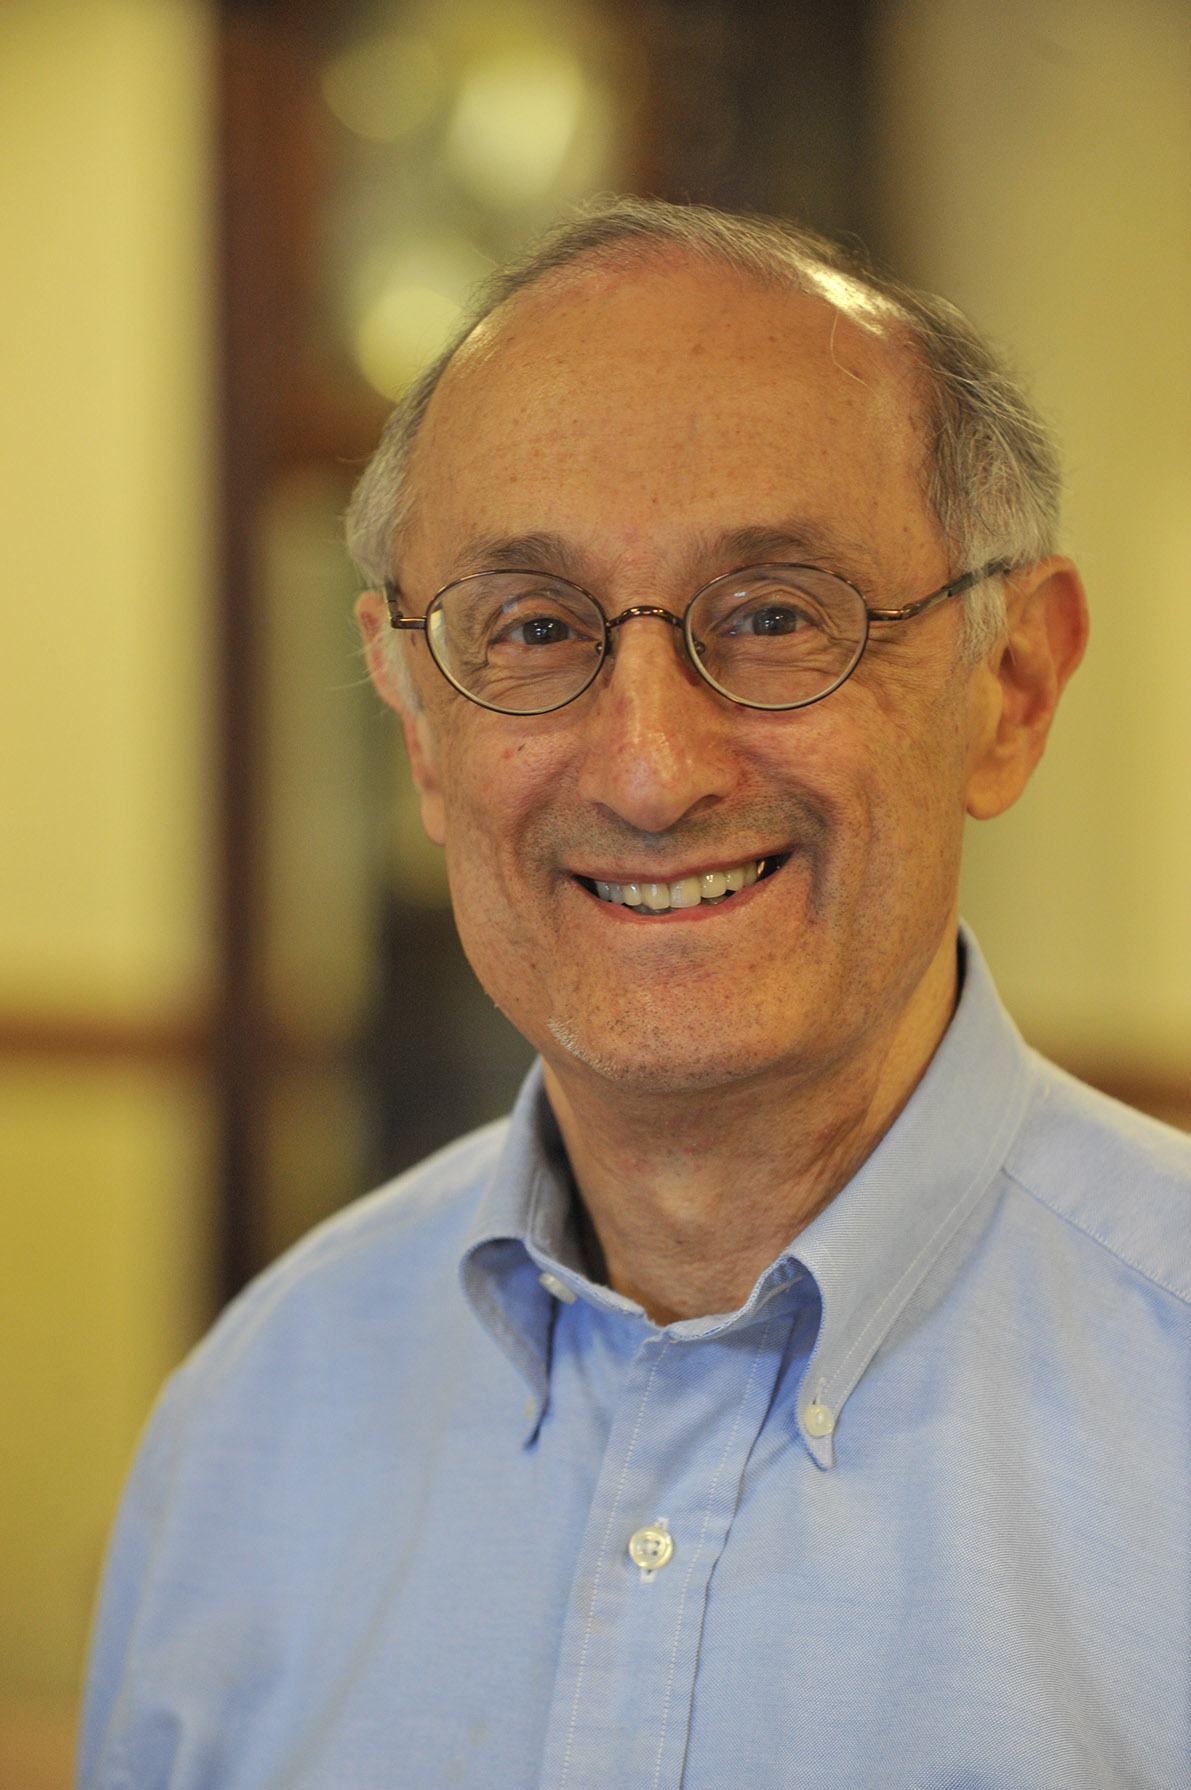
\includegraphics[width=.4\textwidth]{Axelrod}
\end{frame}

\begin{frame}
    \centering
    \includegraphics[width=\textwidth]{strategies}
\end{frame}

\begin{frame}
    \centering
    \huge {\textbf{GOLDEN BALLS}} \\
    \large{\url{https://www.youtube.com/watch?v=p3Uos2fzIJ0}}
\end{frame}

\end{document}
